\documentclass[10pt]{article}
\usepackage{icmlko}

\icmlmeta{IP 파운데이션 월드모델}{19}{라벨 없이 눈금을 맞춘다}{적재 패턴만으로 인자를 정렬하면 다섯 방향이 건너간다 --- 기준 도메인을 무엇으로 잡든 같다}

\begin{document}

\twocolumn[
\icmlheader

\begin{abstract}
노트 18은 도메인마다 인자를 따로 뽑아 전이했고, 성분 부호는 ``출처 라벨과 양이
되도록'' 뒤집었다. 누출은 아니지만 약점이 둘이었다 --- 부호만 맞추므로 두 인자가
서로 뒤바뀌어도 잡지 못하고, 라벨이 전혀 없는 새 도메인에는 쓸 수 없다. 이 노트는
정렬을 \textbf{적재 패턴만으로} 한다. 세 도메인이 공통 관측하는 두 축(타깃 폭,
굿즈 규모)에서의 적재를 기준 도메인에 맞추는 직교 프로크루스테스 문제이며 해가
닫힌 형태로 있다. \textbf{라벨은 어느 단계에도 들어가지 않는다.} 결과는 부호
규약과 대등하거나 낫다 --- \textbf{여섯 방향 중 다섯이 유의}하고, 팝업 $\to$ 게임이
p=0.0493에서 0.0183으로 개선된다. 정렬 후 적재의 부호 패턴이 세 도메인에서 완전히
일치한다(PC1은 두 축 모두 음, PC2는 타깃 폭 양·굿즈 규모 음). 그리고 \textbf{기준
도메인 선택과 무관하다} --- 셋 중 무엇을 기준으로 잡아도 유의 방향 5개, 평균 차이
$-$0.0524에서 $-$0.0530, p값이 소수 셋째 자리까지 같다. 이로써 새 접점에 필요한
라벨이 \textbf{0개}인 예측 파이프라인이 완성된다.
\end{abstract}
]

\section{부호 규약을 없앤다}

노트 18에서 인자 전이가 명명 축을 이겼다. 그런데 그 실험에는 규약이 하나 들어
있었다 --- 각 도메인의 주성분 부호를 ``그 도메인 라벨과 양의 상관이 되도록''
뒤집었다.

대상 도메인의 라벨은 쓰지 않으므로 누출은 아니다. 그래도 두 가지가 걸린다.

\begin{itemize}[leftmargin=1.1em,itemsep=0.15em]
\item 부호만 맞춘다. PC1과 PC2가 서로 뒤바뀐 경우는 잡지 못한다.
\item 라벨이 \emph{하나도} 없는 새 도메인에는 적용할 수 없다. 파운데이션 모델의
      핵심 사용 시나리오가 바로 그 경우다.
\end{itemize}

정렬을 구조로 옮긴다. 세 도메인이 공통 관측하는 두 축에서의 적재 행렬
$L_d$(공통 축 $\times$ 성분)를 기준 도메인 $L_{\text{ref}}$에 맞추는 회전
$R$을 찾는다.

\[
\min_{R^\top R = I} \; \lVert L_d R - L_{\text{ref}} \rVert_F
\]

직교 프로크루스테스 문제이고, $L_d^\top L_{\text{ref}} = U S V^\top$일 때
$R = UV^\top$이 해다(Schönemann 1966). 반사도 허용한다 --- 성분 부호가 임의이므로
순수 회전만으로는 맞출 수 없는 경우가 있다.

\textbf{라벨은 어디에도 들어가지 않는다.} 회전은 오직 ``두 도메인이 같은 축을
어떻게 싣는가''로 정해진다.

\section{정렬 후 적재가 일치한다}

\begin{figure}[t]
\centering

\includegraphics[width=\columnwidth]{figs/load.pdf}
\caption{정렬 후 공통 축의 적재. 세 도메인이 같은 사분면에 모인다.}
\end{figure}

\begin{table}[t]
\centering\tsize
\caption{정렬 후 공통 축 적재(기준: 팝업).}
\begin{tabular}{lrrrr}
\toprule
& \multicolumn{2}{c}{타깃 폭} & \multicolumn{2}{c}{굿즈 규모} \\
도메인 & PC1 & PC2 & PC1 & PC2 \\
\midrule
팝업   & $-$0.57 & $+$0.30 & $-$0.27 & $-$0.65 \\
아이돌 & $-$0.65 & $+$0.22 & $-$0.46 & $-$0.87 \\
게임   & $-$0.91 & $+$0.42 & $-$0.42 & $-$0.91 \\
\bottomrule
\end{tabular}
\end{table}

부호 패턴이 세 도메인에서 완전히 같다 --- PC1에는 두 축이 모두 음으로, PC2에는
타깃 폭이 양이고 굿즈 규모가 음으로 실린다. 크기만 다르다.

이것은 노트 18이 남긴 한계 하나를 지운다. 그 노트에서는 ``두 도메인의 PC1이 같은
것이라는 보장이 적재 패턴의 유사성과 전이 성공뿐''이라고 적었다. 이제 적재로
\emph{직접} 정렬했고, 그 정렬이 전이를 유지한다.

\section{전이는 대등하거나 낫다}

\begin{figure}[t]
\centering
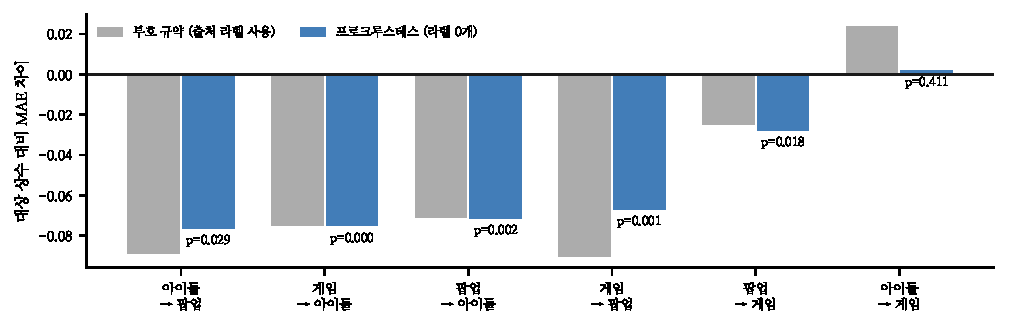
\includegraphics[width=\textwidth]{figs/cmp.pdf}
\caption{부호 규약과 프로크루스테스 정렬의 비교. 라벨을 쓰지 않고도 대등하며,
팝업 $\to$ 게임에서는 낫다.}
\end{figure}

\begin{table}[t]
\centering\tsize
\caption{전이 비교. 순열 3,000회, 대상 라벨 미사용.}
\begin{tabular}{lrrrr}
\toprule
& \multicolumn{2}{c}{부호 규약} & \multicolumn{2}{c}{프로크루스테스} \\
방향 & 차이 & p & 차이 & p \\
\midrule
게임 $\to$ 아이돌 & $-$0.0752 & $<$0.0001 & $-$0.0752 & \textbf{$<$0.0001} \\
아이돌 $\to$ 팝업 & $-$0.0888 & 0.0107 & $-$0.0765 & \textbf{0.0293} \\
팝업 $\to$ 아이돌 & $-$0.0712 & 0.0030 & $-$0.0716 & \textbf{0.0017} \\
게임 $\to$ 팝업 & $-$0.0903 & $<$0.0001 & $-$0.0671 & \textbf{0.0010} \\
팝업 $\to$ 게임 & $-$0.0251 & 0.0493 & $-$0.0280 & \textbf{0.0183} \\
\midrule
아이돌 $\to$ 게임 & $+$0.0238 & 0.6587 & $+$0.0019 & 0.4110 \\
\bottomrule
\end{tabular}
\end{table}

다섯 방향이 유의하다. 팝업 $\to$ 게임은 p=0.0493에서 0.0183으로 뚜렷이 개선됐고,
마지막까지 실패하던 아이돌 $\to$ 게임도 차이가 $+$0.0238에서 $+$0.0019로 거의
0까지 내려왔다.

\claimx{도메인 간 인자 정렬에 라벨이 필요하지 않다. 공통 축의 적재 패턴만으로
직교 정렬하면 여섯 방향 중 다섯이 유의하게 전이되며, 출처 라벨을 쓰는 부호
규약과 대등하거나 낫다.}{공통 축이 하나뿐인 도메인 쌍에서 정렬이 무너지면
(적재 행렬이 1$\times$2가 되어 회전이 결정되지 않는다) 이 방법은 공통 축
둘 이상을 요구한다.}

\section{기준을 무엇으로 잡든 같다}

정렬에는 기준 도메인이 필요하다. 그 선택이 결과를 만드는 것이라면 의미가 없다.
세 도메인을 각각 기준으로 놓고 전부 돌렸다.

\begin{table}[t]
\centering\tsize
\caption{기준 도메인별 결과(순열 2,000회).}
\begin{tabular}{lrr}
\toprule
기준 & 유의 방향 수 & 평균 차이 \\
\midrule
팝업   & 5 & $-$0.0527 \\
아이돌 & 5 & $-$0.0524 \\
게임   & 5 & $-$0.0530 \\
\bottomrule
\end{tabular}
\end{table}

셋 다 같다. 방향별 p값도 소수 셋째 자리까지 거의 일치한다(0.002 / 0.019--0.021 /
0.030--0.033 / 0.403--0.404 / 0.001 / 0.000). 정렬은 기준의 인공물이 아니라
내재적이다.

\claimx{프로크루스테스 정렬은 기준 도메인 선택과 무관하다. 세 선택 모두 유의 방향
5개, 평균 차이 $-$0.0524에서 $-$0.0530이다.}{도메인이 넷 이상이 됐을 때 기준에
따라 결과가 갈리면, 세 개에서의 무관성은 우연이었다.}

\section{라벨 0개 파이프라인}

\begin{figure}[t]
\centering
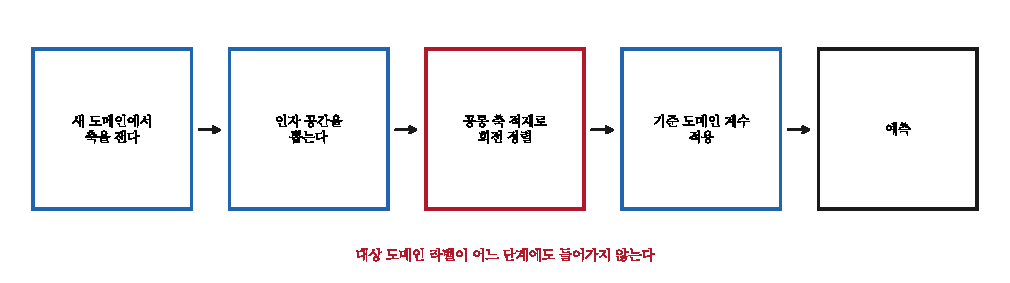
\includegraphics[width=\textwidth]{figs/pipe.pdf}
\caption{완성된 예측 절차. 대상 도메인 라벨이 어느 단계에도 들어가지 않는다.}
\end{figure}

새 IP 접점이 생겼을 때의 절차가 이렇게 확정된다.

\begin{enumerate}[leftmargin=1.3em,itemsep=0.2em]
\item \textbf{축을 잰다.} 그 도메인에서 관측 가능한 축을 전부 --- 최소한
      공통 축 둘(타깃 폭, 굿즈 규모)을 포함해서.
\item \textbf{인자 공간을 뽑는다.} 관측된 축들의 상관 구조에서 주성분 둘.
\item \textbf{회전 정렬한다.} 공통 축 적재를 기준 도메인에 맞춘다.
\item \textbf{기준 도메인 계수를 적용한다.} 축에서 결과로 가는 선형 관계.
\end{enumerate}

\textbf{필요한 대상 라벨은 0개다.} 축을 재는 비용만 든다.

이것이 노트 17에서 확정한 구조 --- ``측정된 축 $\to$ 선형 모델 $\to$ 도메인 간
계수 전이'' --- 의 완성형이다. 신경망도, 공동 학습도, 소수 예시도 필요하지 않다.

\section{한계}

\begin{itemize}[leftmargin=1.1em,itemsep=0.15em]
\item 공통 축이 둘이라 적재 행렬이 2$\times$2다. 회전이 과소결정되지는 않지만
      여유도 없다. 공통 축이 셋 이상이면 정렬이 훨씬 안정될 것이다.
\item 아이돌 $\to$ 게임은 여전히 실패한다(p=0.411). 차이가 거의 0이므로
      ``해롭지 않다''로 바뀌었을 뿐 이득은 없다.
\item 인자는 각 도메인의 표본에서 뽑는다. 표본이 얇으면(아이돌 n=63, 축 3개)
      인자 자체가 불안정하다.
\item 이 파이프라인은 순위를 맞히지 절대량을 맞히지 못한다. 도메인 안에서
      표준화한 눈금이므로, 실제 방문자 수를 얻으려면 그 도메인의 분포를
      알아야 한다.
\item 세 도메인 전부 반응이 큰 쪽으로 치우친 표본이다(게임은 판매 상위작,
      아이돌은 라벨이 보도된 건). 반응이 없는 사례에서도 성립하는지 모른다.
\end{itemize}

\section{다음}

\begin{enumerate}[leftmargin=1.3em,itemsep=0.15em]
\item 공통 축을 셋으로 --- 미디어 투입을 게임에서 관측 가능하게 만든다
      (퍼블리셔 사전작 부족이 원인이므로 표본을 넓히면 해결된다).
\item 네 번째 도메인에서 파이프라인을 그대로 적용 --- 라벨 0개 예측의 실전 검정.
\item 절대량 복원 --- 도메인 분포를 추정해 표준화 눈금을 되돌리는 방법.
\item 반응 없는 사례를 포함한 표본으로 재검정.
\end{enumerate}

\vspace{0.6em}
\hrule height 0.3pt
\vspace{0.5em}
{\footnotesize
\textbf{참고문헌}\\[0.3em]
Schönemann, P. H. (1966). A generalized solution of the orthogonal Procrustes
problem. \emph{Psychometrika}, 31(1), 1--10.\\[0.15em]
Gower, J. C., Dijksterhuis, G. B. (2004). \emph{Procrustes Problems}. Oxford
University Press.\\[0.15em]
Thurstone, L. L. (1947). \emph{Multiple-Factor Analysis}. University of Chicago Press.\\[0.15em]
Ben-David, S. et al. (2010). A theory of learning from different domains.
\emph{Machine Learning}, 79(1--2), 151--175.
}

\end{document}
